\documentclass[english,xcolor=pdftex,dvipsnames,table]{beamer}

\usepackage[T1]{fontenc}
\usepackage[utf8]{inputenc}

\usetheme[informal]{s3it}
\usepackage{s3it}

\title[Introduction to Python]{%
  Using Jupyter Notebooks
}
\author[R.~Murri]{%
  Riccardo Murri \texttt{<riccardo.murri@uzh.ch>}, \\
  Joel Lüthi \texttt{<joel.luethi@uzh.ch>}
  \\
  Pelkmans Lab,
  \\
  University of Zurich
}
\date{October 11, 2018}


\begin{document}

% title frame
\maketitle

\begin{frame}[fragile]
  \frametitle{Outline of the rest of the day}

  \begin{itemize}
    \color{gray}
  \item  9:20 -- 10:00	Upload data to TissueMaps \& start processing it
  \item 10:20 -- 11:30	Image processing \& cell segmentation in TissueMaps
  \item 12:30 -- 13:15	Using machine learning \& downloading data
    \color{black}
  \item 13:30 -- 14:00	Intro to Python
  \item 14:00 -- 14:45	Data processing
  \item 14:45 -- 15:00	Discussing data processing
  \item 15:15 -- 16:00	Plotting data
  \item 16:00 -- 16:30	Discussing plotting \& wrap up
  \end{itemize}
\end{frame}


\begin{frame}
  \frametitle{Jupyter Notebook server}
  \begin{center}
    {\huge\ttfamily http://172.23.{\em X.Y}:2000/}

    \+
    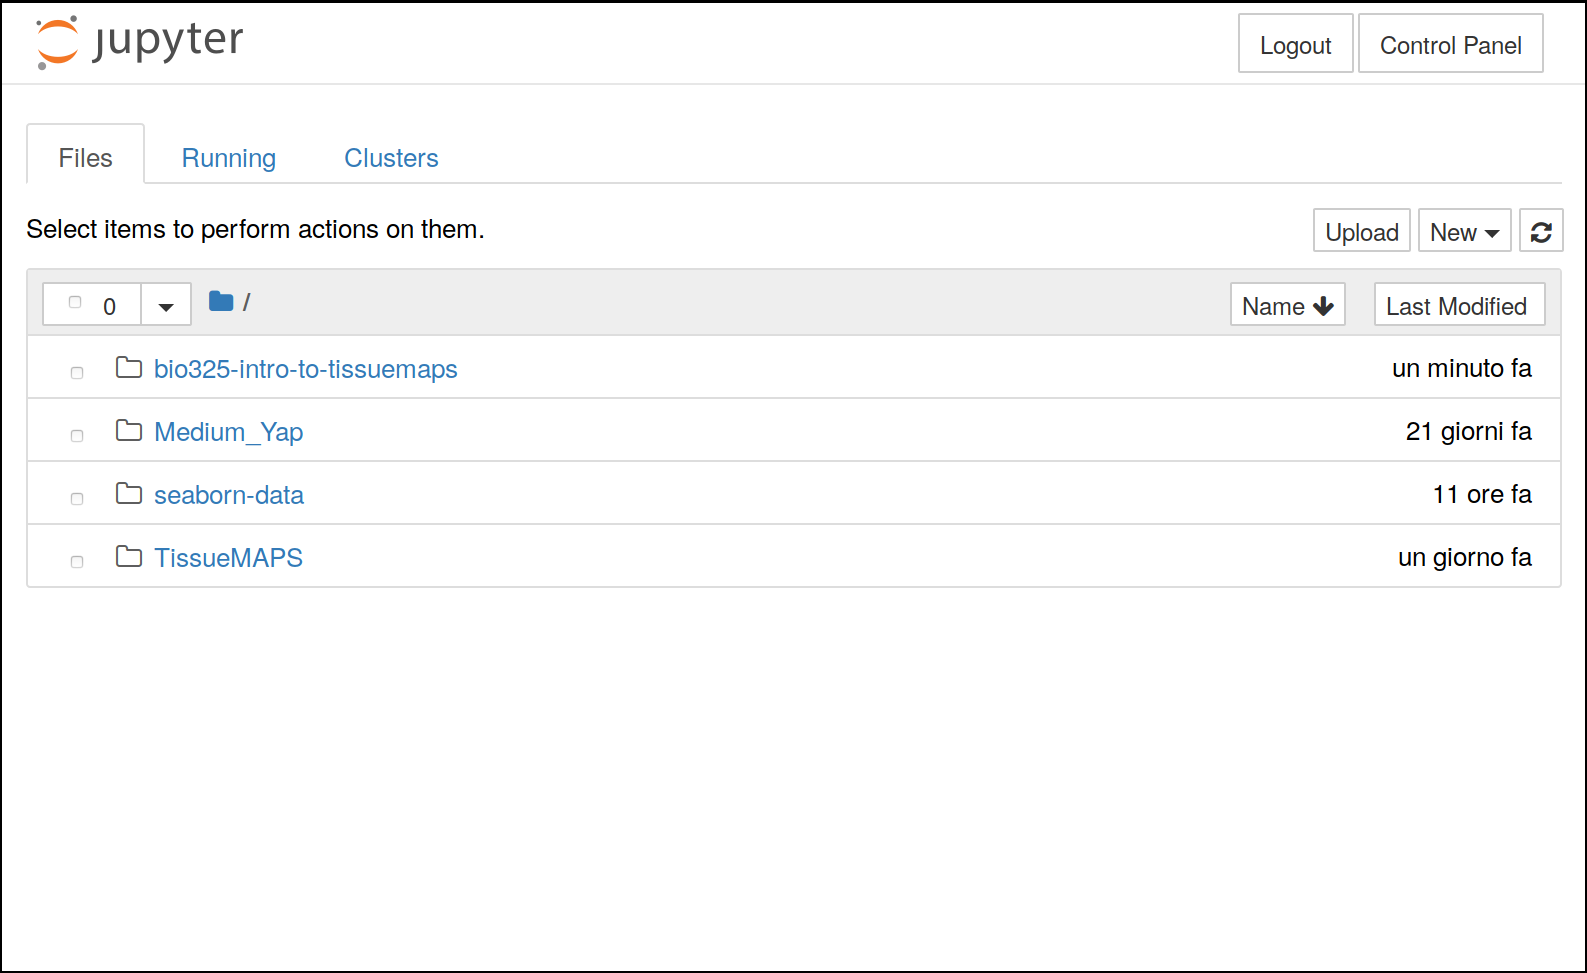
\includegraphics[width=0.75\linewidth]{fig/jupyter.png}

    \+\bf
    Click on the \texttt{python-basics.ipynb} to start.
\end{center}
\end{frame}


\begin{frame}
  \frametitle{The IPython notebook, I}

  \begin{columns}[t]
    \begin{column}{0.5\textwidth}
      \begin{center}
        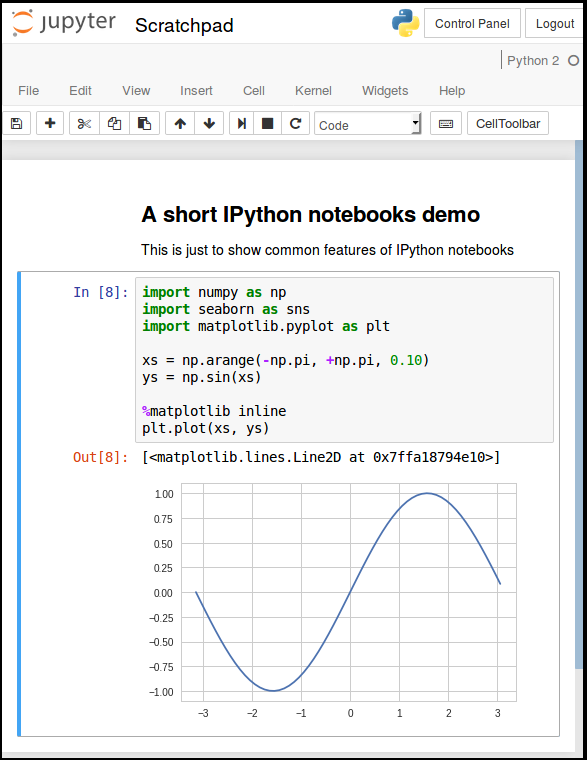
\includegraphics[width=1.00\linewidth]{fig/nb.png}
      \end{center}
    \end{column}
    \begin{column}{0.5\textwidth}
      \small

      A convenient way of interacting with Python is through the IPython
      notebooks.

      \+
      Notebooks are made of ``cells'', which come in two flavors:
      \begin{itemize}
      \item documentation cells, containing text formatted according to the
        \href{http://commonmark.org/help/}{Markdown} conventions;
      \item code cells, containing arbitrary Python code
      \end{itemize}
    \end{column}
  \end{columns}
\end{frame}


\begin{frame}
  \frametitle{The IPython notebook, II}

  To run Python code in the notebook:
  \begin{itemize}
  \item Type your code in a cell besides the {\ttfamily\bfseries\color{blue}
      In~[~]:} (multiple lines are allowed)
  \item Press \textbf{Ctrl+Enter} to evaluate the cell (prompt changes to
    {\ttfamily\bfseries\color{blue} In~[*]:}) --- or press \textbf{Alt+Enter} to
    evaluate the code \emph{and} open a new code cell.
  \item When the Python kernel has done computing, the result appears \emph{under} the
    code cell marked with a {\ttfamily\bfseries\color{red} Out~[~]:} label.
  \end{itemize}
\end{frame}


%\begin{frame}
%   \frametitle{Prerequisites}
%   This course assumes some familiarity with computer programming,
%   and basic knowledge of the Python programming language.

%   \+
%   (You should probably refresh the contents of BIO 134.)
% \end{frame}


\end{document}

%%% Local Variables:
%%% mode: latex
%%% TeX-master: t
%%% End:
